\documentclass[../main.tex]{subfiles}
\begin{document}

\chapter*{PHỤ LỤC: KIẾN TRÚC HỆ THỐNG SRAH}
\addcontentsline{toc}{chapter}{PHỤ LỤC: KIẾN TRÚC HỆ THỐNG SRAH}

Phụ lục này trình bày chi tiết về kiến trúc và cơ chế hoạt động của hệ thống \textbf{SRAH (Security Response \& Analysis Hub)}. Trong khuôn khổ của luận văn, hệ thống SRAH đóng vai trò là một mô hình đối chứng (baseline model), đại diện cho lớp các thuật toán phân phối biên đa lớp (multi-sensor marginal models) được xây dựng chuyên biệt cho bài toán phát hiện bất thường trên Windows.

Mặc dù SRAH không giải quyết được triệt để vấn đề "Nghịch lý cấu trúc" (do bản chất vẫn phân tích trên các cảm biến riêng lẻ thay vì tính toán mật độ đồng thời toàn cục), hệ thống này thể hiện sự tối ưu hóa kỹ thuật vượt trội trong việc xử lý khối lượng lớn dữ liệu \texttt{.evtx} thông qua thiết kế pipeline hiệu năng cao.

\section*{1. Sơ đồ kiến trúc Pipeline của SRAH}

Hệ thống SRAH được thiết kế thành một chuỗi luồng xử lý (pipeline) nhiều lớp, kết hợp ngôn ngữ lập trình Rust để tăng tốc độ nạp dữ liệu và Python để linh hoạt trong phân tích học máy.

\begin{figure}[H]
\centering
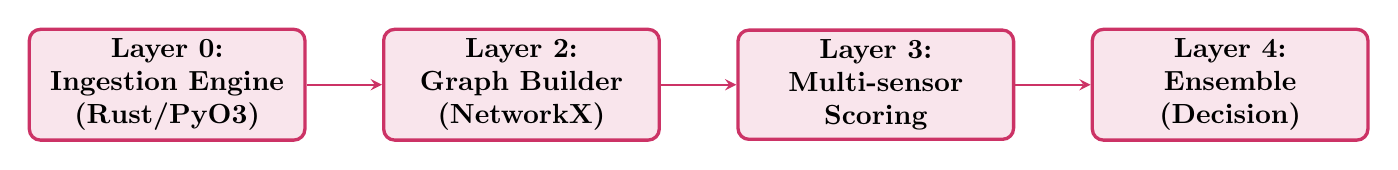
\begin{tikzpicture}[
    node distance=2.5cm,
    layer_box/.style={rectangle, rounded corners, draw=purple!80, fill=purple!10, very thick, minimum width=3.5cm, minimum height=1.2cm, align=center, font=\bfseries},
    arrow/.style={->, >=stealth, thick, purple!80}
]
    % Nodes
    \node[layer_box] (layer0) {Layer 0:\\Ingestion Engine\\(Rust/PyO3)};
    \node[layer_box, right of=layer0, xshift=2.0cm] (layer2) {Layer 2:\\Graph Builder\\(NetworkX)};
    \node[layer_box, right of=layer2, xshift=2.0cm] (layer3) {Layer 3:\\Multi-sensor\\Scoring};
    \node[layer_box, right of=layer3, xshift=2.0cm] (layer4) {Layer 4:\\Ensemble\\(Decision)};

    % Arrows
    \draw[arrow] (layer0) -- (layer2);
    \draw[arrow] (layer2) -- (layer3);
    \draw[arrow] (layer3) -- (layer4);
\end{tikzpicture}
\caption{Sơ đồ kiến trúc Pipeline các lớp của hệ thống SRAH}
\label{fig:srah_pipeline}
\end{figure}

\begin{itemize}
    \item \textbf{Layer 0 (Ingestion Engine):} Thành phần cốt lõi được viết bằng Rust, tối ưu cho việc đọc file \texttt{.evtx} nhị phân với tốc độ cực cao, parse trực tiếp thành các dictionary và chuyển vùng nhớ thẳng vào RAM của Python thông qua bridge \textbf{PyO3}.
    \item \textbf{Layer 2 (Graph Builder):} Xây dựng đồ thị tiến trình (Directed Acyclic Graph) dựa trên trường \texttt{ProcessGuid} thay vì PID nhằm tránh lỗi tái sử dụng PID của Windows.
    \item \textbf{Layer 3 (Multi-sensor Scoring):} Trích xuất đặc trưng và tính toán điểm bất thường độc lập qua 4 cảm biến: Cảm biến điểm (Point), Cảm biến ngữ cảnh (Contextual), Cảm biến chuỗi thời gian (Sequential) và Cảm biến tập thể (Collective).
    \item \textbf{Layer 4 (Ensemble):} Tổng hợp rủi ro từ 4 cảm biến bằng trọng số để đưa ra quyết định cuối cùng.
\end{itemize}

\section*{2. Sơ đồ luồng chạy dữ liệu của SRAH}

Sơ đồ luồng dữ liệu dưới đây chỉ rõ các trạng thái biến đổi của sự kiện từ khi thu thập đến khi xuất ra cảnh báo.

\begin{figure}[H]
\centering
\begin{tikzpicture}[
    node distance=1.8cm,
    data_box/.style={cylinder, shape border rotate=90, draw=teal!80, fill=teal!20, aspect=0.25, thick, minimum width=2.5cm, minimum height=1cm, align=center, font=\small},
    proc_box/.style={rectangle, draw=gray!80, fill=gray!10, thick, minimum width=3.0cm, minimum height=0.8cm, align=center, font=\small},
    arrow/.style={->, >=stealth, thick, gray!80}
]
    % Nodes
    \node[data_box] (evtx) {Sysmon .evtx};
    \node[proc_box, right of=evtx, xshift=2cm] (rust) {Rust Parser};
    \node[data_box, right of=rust, xshift=2cm] (json) {JSON Objects};
    \node[proc_box, right of=json, xshift=2cm] (graph) {Build DAG};
    
    \node[data_box, below of=graph, yshift=-0.5cm] (dag) {Tiến trình (Node)};
    \node[proc_box, left of=dag, xshift=-2cm] (sensor) {Chạy 4 Cảm biến};
    \node[data_box, left of=sensor, xshift=-2cm] (score) {Điểm rủi ro (Score)};

    % Arrows
    \draw[arrow] (evtx) -- (rust);
    \draw[arrow] (rust) -- (json);
    \draw[arrow] (json) -- (graph);
    \draw[arrow] (graph) -- (dag);
    \draw[arrow] (dag) -- (sensor);
    \draw[arrow] (sensor) -- (score);
\end{tikzpicture}
\caption{Sơ đồ luồng chạy dữ liệu (Data Flow) bên trong kiến trúc SRAH}
\label{fig:srah_dataflow}
\end{figure}

Sự tách bạch rõ ràng giữa Engine thu thập tốc độ cao (Rust) và Bộ phân tích ngữ nghĩa (Python) cho phép SRAH vừa đảm bảo tốc độ phản hồi thực tế (Real-time response), vừa có khả năng mở rộng thuật toán phát hiện phức tạp.

\end{document}
